\documentclass[11pt,a4paper]{article}

% ===================== PACKAGES =====================
\usepackage[utf8]{inputenc}
\usepackage[T1]{fontenc}
\usepackage[english]{babel}
\usepackage{amsmath,amssymb,amsthm}
\usepackage{graphicx}
\usepackage{geometry}
\usepackage{booktabs}
\usepackage{xcolor}
\usepackage{hyperref}
\usepackage{caption}
\usepackage{subcaption}
\usepackage{float}
\usepackage{fancyhdr}
\usepackage{enumitem}
\usepackage{tikz}
\usetikzlibrary{arrows.meta,positioning,fit,backgrounds}

\geometry{margin=2.5cm}
\pagestyle{fancy}
\fancyhf{}
\fancyhead[L]{Text-to-Image Generation via Flow Matching}
\fancyhead[R]{\thepage}
\renewcommand{\headrulewidth}{0.4pt}

\hypersetup{
  colorlinks=true,
  linkcolor=blue!50!black,
  citecolor=blue!50!black,
  urlcolor=blue!50!black,
}

\newtheorem{definition}{Definition}
\newtheorem{proposition}{Proposition}

\title{\textbf{Text-Conditioned Image Generation\\ via \emph{Flow Matching}}\\[0.3em]
\large Model Architecture and Results on Colored MNIST}
\author{Technical Report}
\date{2026}

\begin{document}

\maketitle

\begin{abstract}
\noindent
This report presents a text-to-image generative model trained end-to-end: a
cross-attention conditioned \emph{U-Net} guided by a Transformer text
encoder, optimized with the \textbf{flow matching} objective (a simple and
efficient alternative to denoising diffusion probabilistic models). The
model is trained on a synthetic image-captioning task built from colored,
rotated digits. We present the mathematical formulation of flow matching,
the architecture of the network, and the empirical results obtained from a
full training run (loss curves, denoising trajectories, generated samples).
\end{abstract}

\tableofcontents

% ============================================================
\section{Introduction}
% ============================================================

The goal of this work is to study, at a small and tractable scale, the core
mechanisms behind modern text-to-image diffusion/flow models (Stable
Diffusion, Imagen, etc.): a text encoder that turns a natural-language
caption into a conditioning signal, and an image generator that turns that
conditioning signal, together with a continuous notion of time, into a
plausible image.

The task chosen for experimentation is generating colored, rotated
handwritten digits from a free-form textual description of their color,
digit identity, and rotation angle, for example a caption such as
\begin{center}
\textit{"a red 7 rotated 90 degrees"}.
\end{center}

Three components are involved:
\begin{enumerate}
  \item a text encoder that maps a caption to a sequence of contextual
        embeddings (Section~\ref{sec:archi});
  \item an image generator conditioned on that text context via
        cross-attention (Section~\ref{sec:archi});
  \item a \emph{flow matching} training objective, a simple and effective
        alternative to classical DDPM training (Section~\ref{sec:flow}).
\end{enumerate}

% ============================================================
\section{Model Architecture}
\label{sec:archi}
% ============================================================

The model combines two sub-networks: a \textbf{text encoder} (Transformer)
producing a sequential context, and a conditioned \textbf{U-Net} that
predicts, at every timestep $t$, the flow matching velocity field
(Section~\ref{sec:flow}).

\begin{figure}[H]
\centering
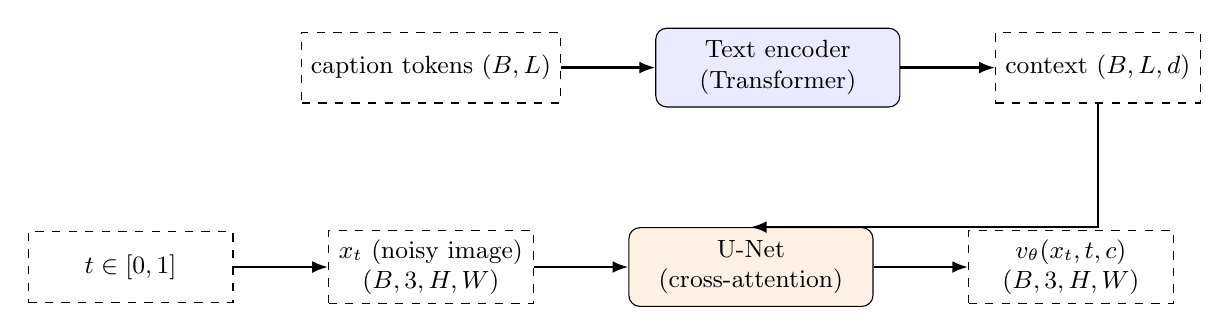
\begin{tikzpicture}[
  node distance=10mm and 12mm,
  block/.style={rectangle, draw, rounded corners, minimum width=3.1cm, minimum height=1.0cm, align=center, font=\small},
  io/.style={rectangle, draw, dashed, minimum width=2.6cm, minimum height=0.9cm, align=center, font=\small},
  arr/.style={-{Latex[length=2mm]}, thick}
]
  \node[io] (tokens) {caption tokens $(B,L)$};
  \node[block, right=of tokens, fill=blue!8] (txtenc) {Text encoder\\(Transformer)};
  \node[io, right=of txtenc] (context) {context $(B,L,d)$};

  \node[io, below=16mm of tokens] (xt) {$x_t$ (noisy image)\\$(B,3,H,W)$};
  \node[io, left=of xt] (t) {$t \in [0,1]$};

  \node[block, right=of xt, fill=orange!10, minimum width=3.1cm] (unet) {U-Net\\(cross-attention)};

  \node[io, right=of unet] (vpred) {$v_\theta(x_t,t,c)$\\$(B,3,H,W)$};

  \draw[arr] (tokens) -- (txtenc);
  \draw[arr] (txtenc) -- (context);
  \draw[arr] (t) -- (xt);
  \draw[arr] (xt) -- (unet);
  \draw[arr] (context.south) |- (unet.north);
  \draw[arr] (unet) -- (vpred);
\end{tikzpicture}
\caption{Model overview: the text encoder produces a sequential context
$c=(B,L,d)$ consumed via cross-attention inside the U-Net, which predicts the
velocity field $v_\theta(x_t, t, c)$ from the noisy image $x_t$ and the
timestep $t$.}
\label{fig:archi-overview}
\end{figure}

\subsection{Text Encoder}

The caption is first mapped to a fixed-length sequence of token indices from
a small closed vocabulary (describing color, digit, and rotation angle), and
padded to a maximum sequence length. This token sequence is then encoded
into a dense contextual representation by:

\begin{enumerate}
  \item an embedding layer mapping each token index to a vector in
        $\mathbb{R}^{d}$;
  \item a learned positional encoding, added elementwise;
  \item a stack of standard Transformer encoder layers (self-attention +
        feed-forward, GELU activation, multi-head attention), which ignore
        padding positions via an attention mask;
  \item a final layer normalization.
\end{enumerate}

The output is a context $c \in \mathbb{R}^{B \times L \times d}$ — a
\emph{per-token} representation rather than a single pooled vector — which
allows the image generator to perform token-level cross-attention, similarly
to how Stable Diffusion conditions on CLIP text embeddings.

\subsection{Time Embedding}

The continuous time variable $t \in [0,1]$ is embedded with a sinusoidal
embedding (as in Transformers / DDPM):
\[
  e(t) = \big[\sin(t f_1), \dots, \sin(t f_{d/2}), \cos(t f_1), \dots,
  \cos(t f_{d/2})\big], \qquad
  f_k = \exp\!\Big(-k \cdot \frac{\ln(10000)}{d/2 - 1}\Big),
\]
then refined by a small multilayer perceptron (linear $\to$ SiLU $\to$
linear, with an expansion factor). The resulting embedding $t_{\mathrm{emb}}$
is injected into every residual block of the U-Net, giving the network
access to the current position along the flow.

\subsection{Conditioned U-Net}

The image generator follows a classical encoder–bottleneck–decoder U-Net
layout with skip connections, operating over multiple spatial resolutions:

\begin{itemize}
  \item \textbf{Residual block}: group normalization $\to$ SiLU $\to$
        $3\times3$ convolution, injection of the projected time embedding
        $t_{\mathrm{emb}}$ between the two convolutions, then group
        normalization $\to$ SiLU $\to$ $3\times3$ convolution again, plus a
        residual connection (with a $1\times1$ convolution when the number
        of channels changes).
  \item \textbf{Downsampling path}: residual blocks followed by
        stride-2 convolutions that halve the spatial resolution at each
        stage while doubling the channel count.
  \item \textbf{Bottleneck}: residual block $\to$ \textbf{cross-attention}
        $\to$ residual block, at the lowest spatial resolution, where the
        quadratic cost of attention (in the number of spatial positions)
        remains small.
  \item \textbf{Upsampling path}: transposed convolutions to double the
        resolution, concatenation with the skip connection from the
        symmetric downsampling stage, then a residual block to fuse the
        two.
  \item \textbf{Output head}: group normalization $\to$ SiLU $\to$
        $3\times3$ convolution back to the image's channel count (predicting
        the velocity field, with the same shape as the input image).
\end{itemize}

\paragraph{Cross-attention block.} This block conditions the spatial feature
map on the text context: the feature map $h \in \mathbb{R}^{B\times C\times
H\times W}$ is flattened into a sequence of pseudo-tokens $(B, HW, C)$,
which queries the text context $c \in \mathbb{R}^{B\times L\times d}$
(used as keys and values) via multi-head attention — the same mechanism used
in Stable Diffusion to condition a U-Net on CLIP text embeddings. The
attention output is added back (residual connection) to the feature map
before the block's second convolution.

\begin{figure}[H]
\centering
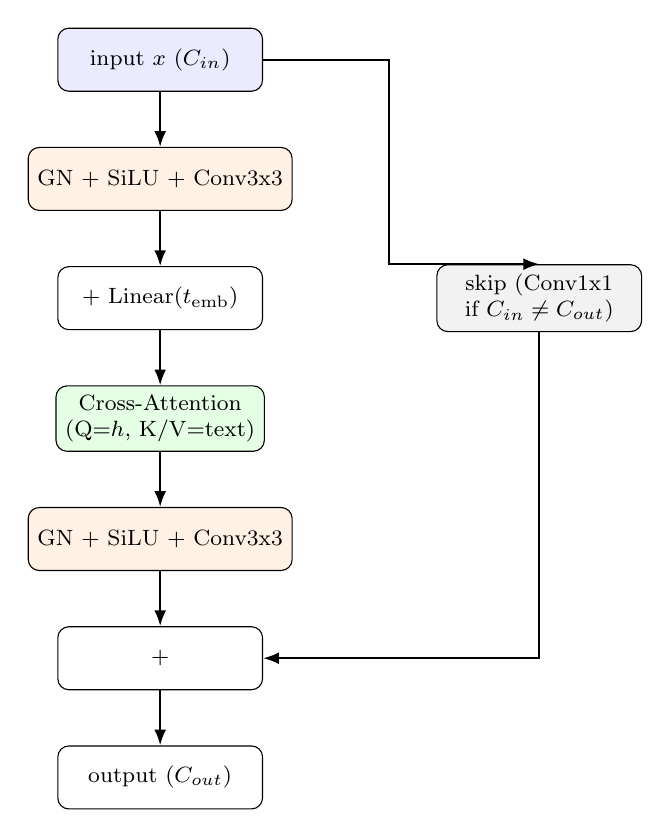
\begin{tikzpicture}[
  node distance=7mm and 10mm,
  block/.style={rectangle, draw, rounded corners, minimum width=2.6cm, minimum height=0.8cm, align=center, font=\footnotesize},
  arr/.style={-{Latex[length=2mm]}, thick}
]
  \node[block, fill=blue!8] (in) {input $x$ ($C_{in}$)};
  \node[block, below=of in, fill=orange!10] (b1) {GN + SiLU + Conv3x3};
  \node[block, below=of b1] (tinj) {$+\ \mathrm{Linear}(t_{\mathrm{emb}})$};
  \node[block, below=of tinj, fill=green!10] (attn) {Cross-Attention\\(Q=$h$, K/V=text)};
  \node[block, below=of attn, fill=orange!10] (b2) {GN + SiLU + Conv3x3};
  \node[block, right=22mm of tinj, fill=gray!10] (skip) {skip (Conv1x1\\ if $C_{in}\neq C_{out}$)};
  \node[block, below=of b2] (sum) {$+$};
  \node[block, below=of sum] (out) {output ($C_{out}$)};

  \draw[arr] (in) -- (b1);
  \draw[arr] (b1) -- (tinj);
  \draw[arr] (tinj) -- (attn);
  \draw[arr] (attn) -- (b2);
  \draw[arr] (b2) -- (sum);
  \draw[arr] (in.east) -- ++(1.6,0) |- (skip.north);
  \draw[arr] (skip.south) |- (sum.east);
  \draw[arr] (sum) -- (out);
\end{tikzpicture}
\caption{Detail of a cross-attention residual block: the time embedding is
injected between the two convolutions (as in a plain residual block), and
cross-attention on the text context is applied before the second
convolution.}
\label{fig:crossattn}
\end{figure}

The resulting network is deliberately compact ($\approx 0.5$M parameters)
compared to production-scale diffusion U-Nets (often $>100$M parameters),
trading generation fidelity for fast training on consumer-grade hardware
while retaining the essential mechanisms: time conditioning, text
cross-attention, and multi-scale skip connections.

% ============================================================
\section{Flow Matching Formulation}
\label{sec:flow}
% ============================================================

\subsection{General Principle}

\emph{Flow matching}~\cite{lipman2023flow} learns a velocity field
$v_\theta(x_t, t)$ that transports, along continuous time $t\in[0,1]$, a
noise sample $x_0 \sim \mathcal{N}(0, I)$ towards a data sample $x_1 \sim
p_{\mathrm{data}}$, following an ordinary differential equation (ODE):
\[
  \frac{dx_t}{dt} = v_\theta(x_t, t), \qquad x_0 \sim \mathcal{N}(0, I)
  \ \longrightarrow\ x_1 \approx \text{image}.
\]

Unlike DDPMs (a stochastic process requiring hundreds of denoising steps),
flow matching directly learns the velocity field of a probability path
chosen \emph{a priori} between noise and data, which makes training
particularly simple: for each training example, a time $t$ and a noise
sample $x_0$ are drawn, the interpolated point $x_t$ and its target velocity
are computed in closed form, and the network is trained to regress that
target velocity.

\subsection{Interpolation Paths}

Two interpolation paths between $x_0$ (noise) and $x_1$ (real data) are
considered:

\begin{description}
  \item[Linear (rectified flow)] Linear interpolation:
    \[
      x_t = (1-t)\,x_0 + t\,x_1, \qquad
      v^{\star}(x_t, t) = \frac{dx_t}{dt} = x_1 - x_0,
    \]
    the target velocity is \textbf{constant in $t$} for a given pair
    $(x_0,x_1)$: this is the \emph{rectified flow}
    path~\cite{liu2023rectifiedflow}, the simplest possible choice (a
    straight line in image space).
  \item[Cosine] Trigonometric interpolation:
    \[
      x_t = \cos\!\Big(\frac{\pi t}{2}\Big) x_0 + \sin\!\Big(\frac{\pi t}{2}\Big) x_1,
      \qquad
      v^{\star}(x_t,t) = \frac{\pi}{2}\Big(\cos\!\Big(\frac{\pi t}{2}\Big) x_1 -
      \sin\!\Big(\frac{\pi t}{2}\Big) x_0\Big),
    \]
    a path along an arc, whose target velocity depends explicitly on $t$
    (accelerating/decelerating near the endpoints).
\end{description}

\subsection{Training Objective}

At each training step, given a batch of real images $x_1$ (normalized to
$[-1,1]$) and their tokenized captions $c$:
\begin{enumerate}
  \item sample noise $x_0 \sim \mathcal{N}(0, I)$ with the same shape as
        $x_1$;
  \item sample a time $t \sim \mathcal{U}(0,1)$, independently per example;
  \item compute $x_t$ and the target velocity $v^\star$ along the chosen
        path;
  \item compute the predicted velocity $v_\theta(x_t, t, c)$ with the
        network;
  \item minimize the mean squared error:
\end{enumerate}
\[
  \mathcal{L}(\theta) = \mathbb{E}_{t\sim\mathcal{U}(0,1),\, x_0\sim\mathcal{N}(0,I),\, (x_1,c)\sim p_{\mathrm{data}}}
  \Big[\ \big\| v_\theta(x_t, t, c) - v^\star(x_t, t) \big\|_2^2\ \Big].
\]

This is a plain MSE regression, with no additional weighting term or KL
divergence — the main source of simplicity of flow matching compared to the
ELBO-based training of DDPMs.

\subsection{Sampling (Inference)}

Image generation consists of numerically integrating the learned ODE,
starting from pure noise, using the explicit Euler method with a constant
step size $\Delta t = 1/N$ over $N$ steps:

\begin{align*}
  x^{(0)} &\sim \mathcal{N}(0, I) \\
  x^{(i+1)} &= x^{(i)} + \Delta t \cdot v_\theta\big(x^{(i)},\, i\Delta t,\, c\big),
  \qquad i = 0, \dots, N-1 \\
  \text{final image} &= \mathrm{clip}(x^{(N)}, -1, 1) \text{ rescaled to } [0,1].
\end{align*}

\begin{figure}[H]
\centering
\begin{minipage}{0.85\textwidth}
\rule{\textwidth}{0.6pt}
\textbf{Algorithm --- Euler Integration Sampling}\\[2pt]
\textit{Input:} model $v_\theta$, caption context $c$, number of steps $N$
\rule{\textwidth}{0.3pt}
\begin{enumerate}[label=\arabic*., itemsep=1pt, topsep=2pt]
  \item $x \gets$ Gaussian noise $\sim \mathcal{N}(0, I)$, image-shaped
  \item $\Delta t \gets 1/N$
  \item \textbf{for} $i = 0$ \textbf{to} $N-1$ \textbf{do}
  \begin{enumerate}[label=(\alph*), itemsep=1pt]
    \item $t \gets i \cdot \Delta t$
    \item $v \gets v_\theta(x, t, c)$ \hfill \textit{// one network forward pass}
    \item $x \gets x + v \cdot \Delta t$ \hfill \textit{// Euler step}
  \end{enumerate}
  \item \textbf{return} $\mathrm{clip}(x, -1, 1)$ rescaled to $[0,1]$
\end{enumerate}
\rule{\textwidth}{0.6pt}
\end{minipage}
\caption{Euler integration sampling procedure.}
\label{alg:sampling}
\end{figure}

The partial image can be recovered after every intermediate step, which is
useful to visualize the denoising trajectory
(Figure~\ref{fig:trajectory}) or to drive an interactive generation
interface.

% ============================================================
\section{Results}
\label{sec:results}
% ============================================================

This section reports results from a complete training run, and samples
generated from the final trained model.

\subsection{Loss Convergence}

Figure~\ref{fig:loss} shows the flow matching MSE loss over the course of
training. The raw per-batch loss (light blue) is overlaid with the
per-epoch average loss (red).

\begin{figure}[H]
\centering
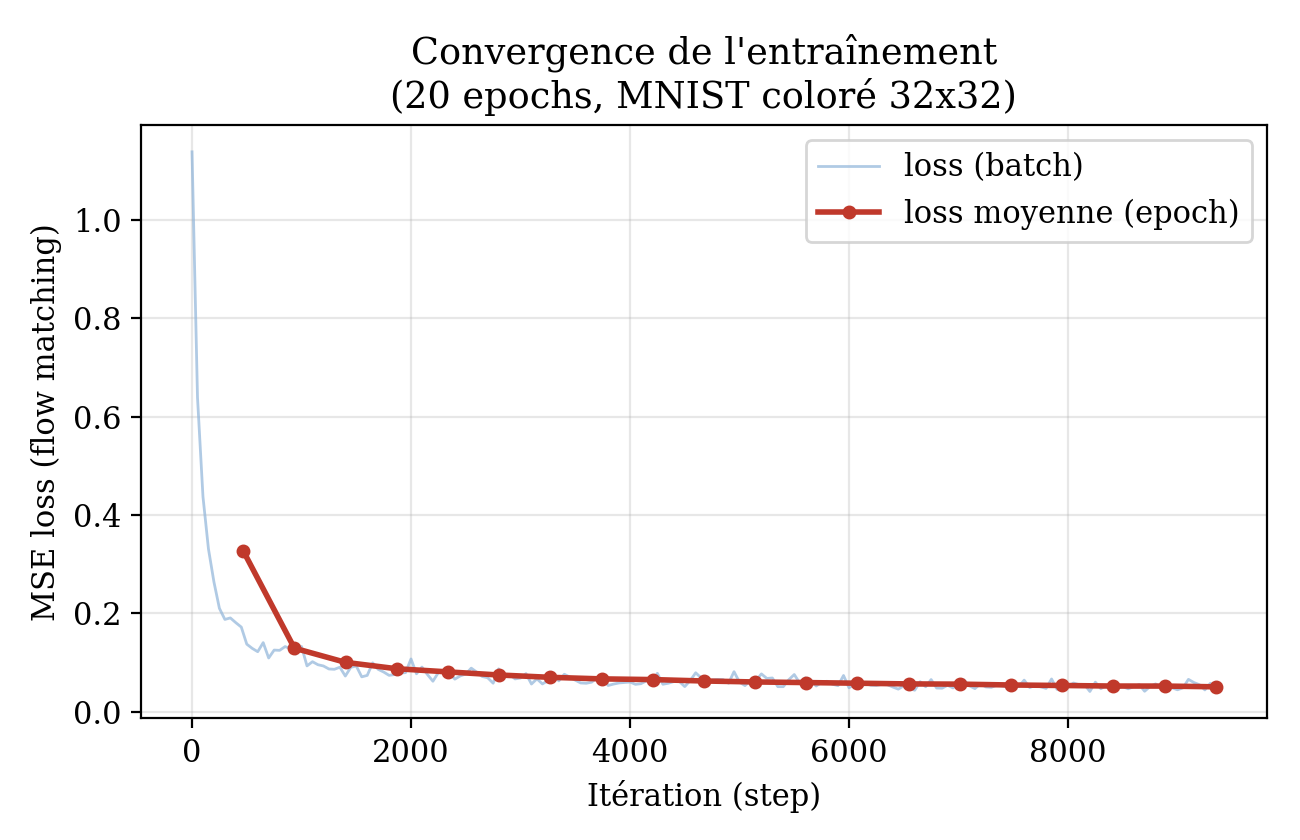
\includegraphics[width=0.85\textwidth]{figures/loss_curve.png}
\caption{Flow matching loss (MSE) over the full training run. The loss drops
sharply within the first epoch ($1.14 \to 0.33$) and then converges
monotonically and smoothly down to $\approx 0.051$.}
\label{fig:loss}
\end{figure}

\begin{table}[H]
\centering
\caption{Average loss per epoch (representative checkpoints).}
\begin{tabular}{@{}rrrrrrrr@{}}
\toprule
Epoch & 1 & 2 & 4 & 8 & 12 & 16 & 20 \\
\midrule
Loss & 0.3273 & 0.1295 & 0.0877 & 0.0657 & 0.0583 & 0.0537 & 0.0510 \\
\bottomrule
\end{tabular}
\end{table}

This is the typical behavior of flow matching training: a very fast decrease
over the first few hundred iterations (the model first learns the global
statistics of the signal — background, dominant hue — the "easy" part of
the target), followed by a slower refinement phase where the model sharpens
the digit's shape and orientation. The curve shows no sign of instability
(no divergence, no oscillation), which validates the choice of the linear
interpolation path and learning rate for this model size.

\subsection{Sampling Trajectory (Denoising)}

Figure~\ref{fig:trajectory} illustrates the ODE integration process
described in Section~\ref{sec:flow}: starting from pure Gaussian noise, the
trained model progressively transforms $x_t$ into a coherent image, for the
caption \textit{"a red 7 rotated 90 degrees"}.

\begin{figure}[H]
\centering
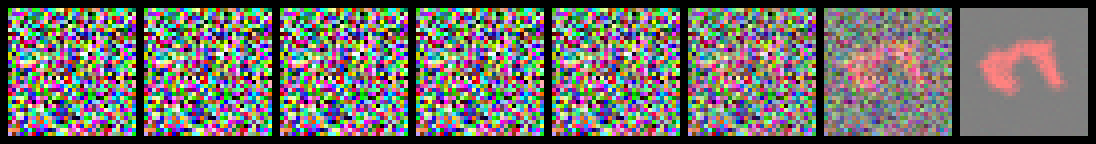
\includegraphics[width=\textwidth]{figures/trajectory_red7_90deg.png}
\caption{Denoising trajectory for the caption \textit{"a red 7 rotated 90
degrees"}, 50-step Euler integration. From left to right: initial noise
($t=0$), intermediate steps ($t \approx 0.02$ to $t \approx 0.70$), and the
final image ($t=1$). Shape and color progressively emerge as $t \to 1$.}
\label{fig:trajectory}
\end{figure}

\subsection{Generated Samples}

Figure~\ref{fig:samples} presents a grid of 12 images generated by the final
trained model, for 12 different combinations of color, digit, and rotation
angle, using 50 integration steps.

\begin{figure}[H]
\centering
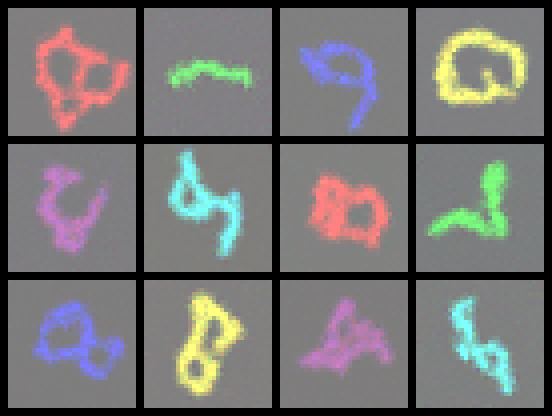
\includegraphics[width=0.6\textwidth]{figures/grid_final_samples.png}
\caption{Samples generated by the trained model, for varied
(color, digit, angle) captions. The model correctly learns the
\textbf{requested color} and an overall \textbf{silhouette} evocative of a
rotated digit, though fine stroke detail remains limited — consistent with
the very small size of the network ($\approx 0.5$M parameters) and the
limited training duration.}
\label{fig:samples}
\end{figure}

\subsection{Qualitative Analysis}

\begin{itemize}
  \item \textbf{Color}: consistently respected — the easiest signal to
        learn (it maps almost bijectively to a single color token in the
        caption), consistent with the rapid loss decrease within the first
        epoch.
  \item \textbf{Digit shape / identity}: partially learned — samples show
        loops and strokes consistent with MNIST digits, without clearly
        reproducing all ten digit classes; this is expected for such a
        small model trained for a limited number of steps.
  \item \textbf{Rotation}: generated silhouettes show varied orientations
        consistent with the angle conditioning, although fine-grained
        control of the exact angle is not visually verifiable at this
        resolution.
  \item \textbf{Sampling stability}: no ODE divergence was observed over the
        50 integration steps; the trajectory stays well-behaved and the
        output remains within $[-1,1]$ after clipping, prior to the final
        affine rescaling to $[0,1]$.
\end{itemize}

These results are consistent with expectations for a small-scale model: the
joint distribution over color, shape, and angle starts to be captured after
a modest training budget on a sub-million-parameter network, which validates
the flow-matching plus cross-attention pipeline end to end.

% ============================================================
\section{Conclusion}
% ============================================================

This report presented a complete text-conditioned image generation model,
trained with the flow matching objective on a colored, rotated digit
generation task. The architecture — a Transformer text encoder combined with
a cross-attention U-Net — faithfully follows the design principles of
production text-to-image diffusion models, at a scale suited to local
experimentation. Training converges stably (loss $1.14 \to 0.051$) and
produces samples that correctly respect the requested color while sketching
the digit's shape and orientation, validating the full pipeline from text
conditioning to iterative ODE-based sampling.

% ============================================================
\begin{thebibliography}{9}

\bibitem{lipman2023flow}
Y.~Lipman, R.~T.~Q.~Chen, H.~Ben-Hamu, M.~Nickel, M.~Le,
\emph{Flow Matching for Generative Modeling}, ICLR 2023.

\bibitem{liu2023rectifiedflow}
X.~Liu, C.~Gong, Q.~Liu,
\emph{Flow Straight and Fast: Learning to Generate and Transfer Data with
Rectified Flow}, ICLR 2023.

\bibitem{ho2020ddpm}
J.~Ho, A.~Jain, P.~Abbeel,
\emph{Denoising Diffusion Probabilistic Models}, NeurIPS 2020.

\bibitem{rombach2022ldm}
R.~Rombach, A.~Blattmann, D.~Lorenz, P.~Esser, B.~Ommer,
\emph{High-Resolution Image Synthesis with Latent Diffusion Models}, CVPR 2022.

\bibitem{vaswani2017attention}
A.~Vaswani et al., \emph{Attention Is All You Need}, NeurIPS 2017.

\end{thebibliography}

\end{document}
